% design and analysis

\section{Design and Analysis}

Use this section for introducing logistic regression. \\
High level...show the function, explain it.

\subsection{Data Transformations and Standardization}

In modeling using logistic regression, the appropriate transformations on continuous variables are necessary to optimize the model predictiveness. \par
Variable transformation is an important technique to create robust models using logistic regression. Because the predictors are linear in the log of the odds, it is often helpful to transform the continuous variables to create a more linear relationship. \par
The raw data collected contained several predictors with high skewness values.
A few concerning features were determined to be PSA Level (skewness = 4.39), Cancer Volume (skewness = 2.18), and Weight (skewness = 7.46). As a prepossessing step to reduce skewness, I elected to transform these continuous predictor variables using the log-transformation, and standardize \textit{all} the data on top of that. The standardization step was used to normalize the data, did not affect any underlying distributions, and was performed by using the following design: \par 

The finalized data skewness is summarized directly below. Following, I've included the histogram of PSA Level vs. Cancer Volume vs. Age, a helpful visual for the three predictors which carried the most significance through much of my analysis.

\begin{center}
	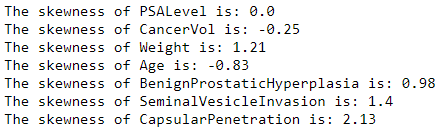
\includegraphics{final_SKEWNESS.png} \\
\end{center}

\begin{center}
	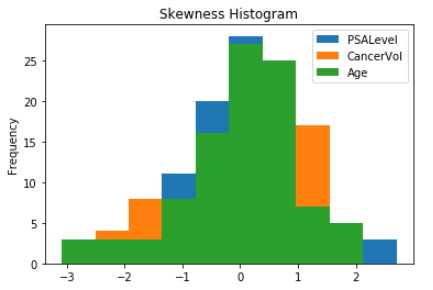
\includegraphics{psa_cancervol_age_SKEWNESS.png}
\end{center}

\subsection{Second order Predictors}

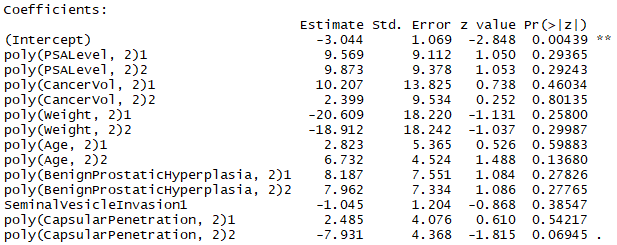
\includegraphics{poly_output}

\subsection{Model Selection}

\subsection{Analysis of Residuals}
\subsubsection{Influential Observations}

\subsection{Goodness Of Fit Evaluation}

\subsection{Development of ROC Curve}
\subsubsection{Prediction Rule}

\subsection{Model: Strengths and Weaknesses}
-discuss correlation matrix \\
-PSALevel and CancerVol show a mild level of correlation: 0.624151